\chapter{Introduction}
\lipsum[1-10]


\printinunitsof{in}\prntlen{\textwidth}


% \begin{figure*}
%   \centering
% \begin{subfigure}{0.3\linewidth}  % <----
%  % This file was created with tikzplotlib v0.10.1.
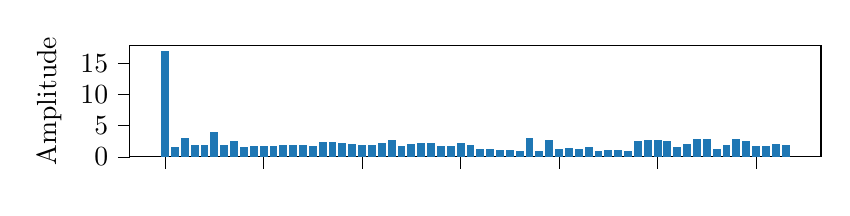
\begin{tikzpicture}

\definecolor{darkgray176}{RGB}{176,176,176}
\definecolor{steelblue31119180}{RGB}{31,119,180}

\begin{axis}[
height=3cm,
scaled x ticks=manual:{}{\pgfmathparse{#1}},
tick align=outside,
tick pos=left,
width=294.76926pt,
x grid style={darkgray176},
xmin=-3.59, xmax=66.59,
xtick style={color=black},
xticklabels={},
y grid style={darkgray176},
ylabel={Amplitude},
ymin=0, ymax=17.9224917606911,
ytick style={color=black},
ytick={0,5,10,15,20},
yticklabels={
  \(\displaystyle {0}\),
  \(\displaystyle {5}\),
  \(\displaystyle {10}\),
  \(\displaystyle {15}\),
  \(\displaystyle {20}\)
}
]
\draw[draw=none,fill=steelblue31119180] (axis cs:-0.4,0) rectangle (axis cs:0.4,17.0690397720867);
\draw[draw=none,fill=steelblue31119180] (axis cs:0.6,0) rectangle (axis cs:1.4,1.57701532870284);
\draw[draw=none,fill=steelblue31119180] (axis cs:1.6,0) rectangle (axis cs:2.4,3.04515592469192);
\draw[draw=none,fill=steelblue31119180] (axis cs:2.6,0) rectangle (axis cs:3.4,1.98727065046711);
\draw[draw=none,fill=steelblue31119180] (axis cs:3.6,0) rectangle (axis cs:4.4,1.87901229043815);
\draw[draw=none,fill=steelblue31119180] (axis cs:4.6,0) rectangle (axis cs:5.4,3.94494985947408);
\draw[draw=none,fill=steelblue31119180] (axis cs:5.6,0) rectangle (axis cs:6.4,1.94821362148988);
\draw[draw=none,fill=steelblue31119180] (axis cs:6.6,0) rectangle (axis cs:7.4,2.53456682074799);
\draw[draw=none,fill=steelblue31119180] (axis cs:7.6,0) rectangle (axis cs:8.4,1.53982779775888);
\draw[draw=none,fill=steelblue31119180] (axis cs:8.6,0) rectangle (axis cs:9.4,1.81855063876657);
\draw[draw=none,fill=steelblue31119180] (axis cs:9.6,0) rectangle (axis cs:10.4,1.74372106320514);
\draw[draw=none,fill=steelblue31119180] (axis cs:10.6,0) rectangle (axis cs:11.4,1.78981913351115);
\draw[draw=none,fill=steelblue31119180] (axis cs:11.6,0) rectangle (axis cs:12.4,1.9283565514217);
\draw[draw=none,fill=steelblue31119180] (axis cs:12.6,0) rectangle (axis cs:13.4,1.98727539890716);
\draw[draw=none,fill=steelblue31119180] (axis cs:13.6,0) rectangle (axis cs:14.4,1.83637697194901);
\draw[draw=none,fill=steelblue31119180] (axis cs:14.6,0) rectangle (axis cs:15.4,1.70629362470728);
\draw[draw=none,fill=steelblue31119180] (axis cs:15.6,0) rectangle (axis cs:16.4,2.32898911515285);
\draw[draw=none,fill=steelblue31119180] (axis cs:16.6,0) rectangle (axis cs:17.4,2.38726500121464);
\draw[draw=none,fill=steelblue31119180] (axis cs:17.6,0) rectangle (axis cs:18.4,2.2146470907513);
\draw[draw=none,fill=steelblue31119180] (axis cs:18.6,0) rectangle (axis cs:19.4,2.08886171015996);
\draw[draw=none,fill=steelblue31119180] (axis cs:19.6,0) rectangle (axis cs:20.4,1.91586717365543);
\draw[draw=none,fill=steelblue31119180] (axis cs:20.6,0) rectangle (axis cs:21.4,1.97741699428014);
\draw[draw=none,fill=steelblue31119180] (axis cs:21.6,0) rectangle (axis cs:22.4,2.26324345140917);
\draw[draw=none,fill=steelblue31119180] (axis cs:22.6,0) rectangle (axis cs:23.4,2.74150949309368);
\draw[draw=none,fill=steelblue31119180] (axis cs:23.6,0) rectangle (axis cs:24.4,1.67879784390802);
\draw[draw=none,fill=steelblue31119180] (axis cs:24.6,0) rectangle (axis cs:25.4,1.99560308046926);
\draw[draw=none,fill=steelblue31119180] (axis cs:25.6,0) rectangle (axis cs:26.4,2.18236194366914);
\draw[draw=none,fill=steelblue31119180] (axis cs:26.6,0) rectangle (axis cs:27.4,2.28116664486001);
\draw[draw=none,fill=steelblue31119180] (axis cs:27.6,0) rectangle (axis cs:28.4,1.76545125094874);
\draw[draw=none,fill=steelblue31119180] (axis cs:28.6,0) rectangle (axis cs:29.4,1.79936118428771);
\draw[draw=none,fill=steelblue31119180] (axis cs:29.6,0) rectangle (axis cs:30.4,2.21046386064049);
\draw[draw=none,fill=steelblue31119180] (axis cs:30.6,0) rectangle (axis cs:31.4,1.92512684988102);
\draw[draw=none,fill=steelblue31119180] (axis cs:31.6,0) rectangle (axis cs:32.4,1.29434219923151);
\draw[draw=none,fill=steelblue31119180] (axis cs:32.6,0) rectangle (axis cs:33.4,1.24905838096159);
\draw[draw=none,fill=steelblue31119180] (axis cs:33.6,0) rectangle (axis cs:34.4,1.0539404131426);
\draw[draw=none,fill=steelblue31119180] (axis cs:34.6,0) rectangle (axis cs:35.4,1.07785302549105);
\draw[draw=none,fill=steelblue31119180] (axis cs:35.6,0) rectangle (axis cs:36.4,1.00170991631713);
\draw[draw=none,fill=steelblue31119180] (axis cs:36.6,0) rectangle (axis cs:37.4,2.990570610034);
\draw[draw=none,fill=steelblue31119180] (axis cs:37.6,0) rectangle (axis cs:38.4,1.00976749017216);
\draw[draw=none,fill=steelblue31119180] (axis cs:38.6,0) rectangle (axis cs:39.4,2.77121989223762);
\draw[draw=none,fill=steelblue31119180] (axis cs:39.6,0) rectangle (axis cs:40.4,1.21267465980989);
\draw[draw=none,fill=steelblue31119180] (axis cs:40.6,0) rectangle (axis cs:41.4,1.44620941204964);
\draw[draw=none,fill=steelblue31119180] (axis cs:41.6,0) rectangle (axis cs:42.4,1.26138331095181);
\draw[draw=none,fill=steelblue31119180] (axis cs:42.6,0) rectangle (axis cs:43.4,1.60664374136418);
\draw[draw=none,fill=steelblue31119180] (axis cs:43.6,0) rectangle (axis cs:44.4,0.883196382772003);
\draw[draw=none,fill=steelblue31119180] (axis cs:44.6,0) rectangle (axis cs:45.4,1.0835546712407);
\draw[draw=none,fill=steelblue31119180] (axis cs:45.6,0) rectangle (axis cs:46.4,1.05267232084);
\draw[draw=none,fill=steelblue31119180] (axis cs:46.6,0) rectangle (axis cs:47.4,0.94061509525324);
\draw[draw=none,fill=steelblue31119180] (axis cs:47.6,0) rectangle (axis cs:48.4,2.5937245360833);
\draw[draw=none,fill=steelblue31119180] (axis cs:48.6,0) rectangle (axis cs:49.4,2.7964850933437);
\draw[draw=none,fill=steelblue31119180] (axis cs:49.6,0) rectangle (axis cs:50.4,2.71286149748853);
\draw[draw=none,fill=steelblue31119180] (axis cs:50.6,0) rectangle (axis cs:51.4,2.61834135486071);
\draw[draw=none,fill=steelblue31119180] (axis cs:51.6,0) rectangle (axis cs:52.4,1.64261763713365);
\draw[draw=none,fill=steelblue31119180] (axis cs:52.6,0) rectangle (axis cs:53.4,2.10765089952882);
\draw[draw=none,fill=steelblue31119180] (axis cs:53.6,0) rectangle (axis cs:54.4,2.79833649937833);
\draw[draw=none,fill=steelblue31119180] (axis cs:54.6,0) rectangle (axis cs:55.4,2.89223762573101);
\draw[draw=none,fill=steelblue31119180] (axis cs:55.6,0) rectangle (axis cs:56.4,1.32361974945306);
\draw[draw=none,fill=steelblue31119180] (axis cs:56.6,0) rectangle (axis cs:57.4,1.84030534558782);
\draw[draw=none,fill=steelblue31119180] (axis cs:57.6,0) rectangle (axis cs:58.4,2.82922380450697);
\draw[draw=none,fill=steelblue31119180] (axis cs:58.6,0) rectangle (axis cs:59.4,2.5822341294544);
\draw[draw=none,fill=steelblue31119180] (axis cs:59.6,0) rectangle (axis cs:60.4,1.71682916120663);
\draw[draw=none,fill=steelblue31119180] (axis cs:60.6,0) rectangle (axis cs:61.4,1.73398491114388);
\draw[draw=none,fill=steelblue31119180] (axis cs:61.6,0) rectangle (axis cs:62.4,2.13866133729592);
\draw[draw=none,fill=steelblue31119180] (axis cs:62.6,0) rectangle (axis cs:63.4,1.90570304888095);
\end{axis}

\end{tikzpicture}

%  \caption{Model 1}
%  \label{fig1a}
% \end{subfigure}

% \begin{subfigure}{0.3\linewidth}  % <----
%  % This file was created with tikzplotlib v0.10.1.
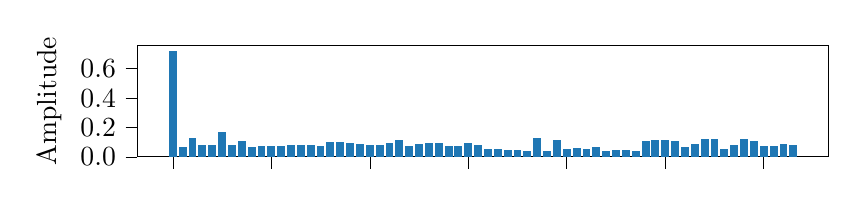
\begin{tikzpicture}

\definecolor{darkgray176}{RGB}{176,176,176}
\definecolor{steelblue31119180}{RGB}{31,119,180}

\begin{axis}[
height=3cm,
scaled x ticks=manual:{}{\pgfmathparse{#1}},
tick align=outside,
tick pos=left,
width=294.76926pt,
x grid style={darkgray176},
xmin=-3.59, xmax=66.59,
xtick style={color=black},
xticklabels={},
y grid style={darkgray176},
ylabel={Amplitude},
ymin=0, ymax=0.75975651477895,
ytick style={color=black},
ytick={0,0.2,0.4,0.6,0.8},
yticklabels={
  \(\displaystyle {0.0}\),
  \(\displaystyle {0.2}\),
  \(\displaystyle {0.4}\),
  \(\displaystyle {0.6}\),
  \(\displaystyle {0.8}\)
}
]
\draw[draw=none,fill=steelblue31119180] (axis cs:-0.4,0) rectangle (axis cs:0.4,0.72357763312281);
\draw[draw=none,fill=steelblue31119180] (axis cs:0.6,0) rectangle (axis cs:1.4,0.06685162341746);
\draw[draw=none,fill=steelblue31119180] (axis cs:1.6,0) rectangle (axis cs:2.4,0.129087912729675);
\draw[draw=none,fill=steelblue31119180] (axis cs:2.6,0) rectangle (axis cs:3.4,0.0842428521369383);
\draw[draw=none,fill=steelblue31119180] (axis cs:3.6,0) rectangle (axis cs:4.4,0.0796536468294661);
\draw[draw=none,fill=steelblue31119180] (axis cs:4.6,0) rectangle (axis cs:5.4,0.167231286599636);
\draw[draw=none,fill=steelblue31119180] (axis cs:5.6,0) rectangle (axis cs:6.4,0.0825871765417374);
\draw[draw=none,fill=steelblue31119180] (axis cs:6.6,0) rectangle (axis cs:7.4,0.10744341132461);
\draw[draw=none,fill=steelblue31119180] (axis cs:7.6,0) rectangle (axis cs:8.4,0.0652751981480014);
\draw[draw=none,fill=steelblue31119180] (axis cs:8.6,0) rectangle (axis cs:9.4,0.0770906028975654);
\draw[draw=none,fill=steelblue31119180] (axis cs:9.6,0) rectangle (axis cs:10.4,0.0739184849638508);
\draw[draw=none,fill=steelblue31119180] (axis cs:10.6,0) rectangle (axis cs:11.4,0.0758726389788938);
\draw[draw=none,fill=steelblue31119180] (axis cs:11.6,0) rectangle (axis cs:12.4,0.0817454108681824);
\draw[draw=none,fill=steelblue31119180] (axis cs:12.6,0) rectangle (axis cs:13.4,0.0842430534291643);
\draw[draw=none,fill=steelblue31119180] (axis cs:13.6,0) rectangle (axis cs:14.4,0.0778462831316993);
\draw[draw=none,fill=steelblue31119180] (axis cs:14.6,0) rectangle (axis cs:15.4,0.0723318897175019);
\draw[draw=none,fill=steelblue31119180] (axis cs:15.6,0) rectangle (axis cs:16.4,0.0987287190148169);
\draw[draw=none,fill=steelblue31119180] (axis cs:16.6,0) rectangle (axis cs:17.4,0.101199105648615);
\draw[draw=none,fill=steelblue31119180] (axis cs:17.6,0) rectangle (axis cs:18.4,0.09388161967662);
\draw[draw=none,fill=steelblue31119180] (axis cs:18.6,0) rectangle (axis cs:19.4,0.088549422365874);
\draw[draw=none,fill=steelblue31119180] (axis cs:19.6,0) rectangle (axis cs:20.4,0.0812159707518103);
\draw[draw=none,fill=steelblue31119180] (axis cs:20.6,0) rectangle (axis cs:21.4,0.0838251435067765);
\draw[draw=none,fill=steelblue31119180] (axis cs:21.6,0) rectangle (axis cs:22.4,0.0959416792987612);
\draw[draw=none,fill=steelblue31119180] (axis cs:22.6,0) rectangle (axis cs:23.4,0.116215966257247);
\draw[draw=none,fill=steelblue31119180] (axis cs:23.6,0) rectangle (axis cs:24.4,0.0711663096815281);
\draw[draw=none,fill=steelblue31119180] (axis cs:24.6,0) rectangle (axis cs:25.4,0.0845960741142504);
\draw[draw=none,fill=steelblue31119180] (axis cs:25.6,0) rectangle (axis cs:26.4,0.092513012501134);
\draw[draw=none,fill=steelblue31119180] (axis cs:26.6,0) rectangle (axis cs:27.4,0.0967014655590507);
\draw[draw=none,fill=steelblue31119180] (axis cs:27.6,0) rectangle (axis cs:28.4,0.0748396544042398);
\draw[draw=none,fill=steelblue31119180] (axis cs:28.6,0) rectangle (axis cs:29.4,0.076277138271662);
\draw[draw=none,fill=steelblue31119180] (axis cs:29.6,0) rectangle (axis cs:30.4,0.0937042873964914);
\draw[draw=none,fill=steelblue31119180] (axis cs:30.6,0) rectangle (axis cs:31.4,0.0816084998393432);
\draw[draw=none,fill=steelblue31119180] (axis cs:31.6,0) rectangle (axis cs:32.4,0.0548687610712862);
\draw[draw=none,fill=steelblue31119180] (axis cs:32.6,0) rectangle (axis cs:33.4,0.0529491242035992);
\draw[draw=none,fill=steelblue31119180] (axis cs:33.6,0) rectangle (axis cs:34.4,0.0446778330695149);
\draw[draw=none,fill=steelblue31119180] (axis cs:34.6,0) rectangle (axis cs:35.4,0.0456915181786893);
\draw[draw=none,fill=steelblue31119180] (axis cs:35.6,0) rectangle (axis cs:36.4,0.0424637179362424);
\draw[draw=none,fill=steelblue31119180] (axis cs:36.6,0) rectangle (axis cs:37.4,0.126773973966228);
\draw[draw=none,fill=steelblue31119180] (axis cs:37.6,0) rectangle (axis cs:38.4,0.0428052884227246);
\draw[draw=none,fill=steelblue31119180] (axis cs:38.6,0) rectangle (axis cs:39.4,0.117475426694316);
\draw[draw=none,fill=steelblue31119180] (axis cs:39.6,0) rectangle (axis cs:40.4,0.0514067734219108);
\draw[draw=none,fill=steelblue31119180] (axis cs:40.6,0) rectangle (axis cs:41.4,0.0613065993953611);
\draw[draw=none,fill=steelblue31119180] (axis cs:41.6,0) rectangle (axis cs:42.4,0.0534715931760668);
\draw[draw=none,fill=steelblue31119180] (axis cs:42.6,0) rectangle (axis cs:43.4,0.0681076083464856);
\draw[draw=none,fill=steelblue31119180] (axis cs:43.6,0) rectangle (axis cs:44.4,0.0374397831841637);
\draw[draw=none,fill=steelblue31119180] (axis cs:44.6,0) rectangle (axis cs:45.4,0.0459332179691593);
\draw[draw=none,fill=steelblue31119180] (axis cs:45.6,0) rectangle (axis cs:46.4,0.0446240770739142);
\draw[draw=none,fill=steelblue31119180] (axis cs:46.6,0) rectangle (axis cs:47.4,0.0398738331734358);
\draw[draw=none,fill=steelblue31119180] (axis cs:47.6,0) rectangle (axis cs:48.4,0.109951179788145);
\draw[draw=none,fill=steelblue31119180] (axis cs:48.6,0) rectangle (axis cs:49.4,0.11854644970796);
\draw[draw=none,fill=steelblue31119180] (axis cs:49.6,0) rectangle (axis cs:50.4,0.115001542415574);
\draw[draw=none,fill=steelblue31119180] (axis cs:50.6,0) rectangle (axis cs:51.4,0.110994717075761);
\draw[draw=none,fill=steelblue31119180] (axis cs:51.6,0) rectangle (axis cs:52.4,0.0696325861251211);
\draw[draw=none,fill=steelblue31119180] (axis cs:52.6,0) rectangle (axis cs:53.4,0.0893459192604471);
\draw[draw=none,fill=steelblue31119180] (axis cs:53.6,0) rectangle (axis cs:54.4,0.118624933091582);
\draw[draw=none,fill=steelblue31119180] (axis cs:54.6,0) rectangle (axis cs:55.4,0.122605517568569);
\draw[draw=none,fill=steelblue31119180] (axis cs:55.6,0) rectangle (axis cs:56.4,0.0561098725090596);
\draw[draw=none,fill=steelblue31119180] (axis cs:56.6,0) rectangle (axis cs:57.4,0.0780128117318752);
\draw[draw=none,fill=steelblue31119180] (axis cs:57.6,0) rectangle (axis cs:58.4,0.119934284023851);
\draw[draw=none,fill=steelblue31119180] (axis cs:58.6,0) rectangle (axis cs:59.4,0.109464087289494);
\draw[draw=none,fill=steelblue31119180] (axis cs:59.6,0) rectangle (axis cs:60.4,0.0727785040945065);
\draw[draw=none,fill=steelblue31119180] (axis cs:60.6,0) rectangle (axis cs:61.4,0.0735057574783992);
\draw[draw=none,fill=steelblue31119180] (axis cs:61.6,0) rectangle (axis cs:62.4,0.090660489937019);
\draw[draw=none,fill=steelblue31119180] (axis cs:62.6,0) rectangle (axis cs:63.4,0.080785100975579);
\end{axis}

\end{tikzpicture}

%  \caption{Model 2}
%  \label{fig1b}
% \end{subfigure}

% \begin{subfigure}{0.3\linewidth}  % <----
%  % This file was created with tikzplotlib v0.10.1.
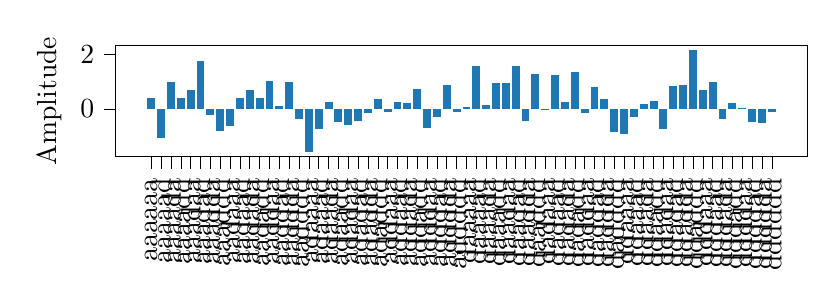
\begin{tikzpicture}

\definecolor{darkgray176}{RGB}{176,176,176}
\definecolor{steelblue31119180}{RGB}{31,119,180}

\begin{axis}[
height=3cm,
tick align=outside,
tick pos=left,
width=294.76926pt,
x grid style={darkgray176},
xmin=-3.59, xmax=66.59,
xtick style={color=black},
xtick={0,1,2,3,4,5,6,7,8,9,10,11,12,13,14,15,16,17,18,19,20,21,22,23,24,25,26,27,28,29,30,31,32,33,34,35,36,37,38,39,40,41,42,43,44,45,46,47,48,49,50,51,52,53,54,55,56,57,58,59,60,61,62,63},
xticklabel style={rotate=90.0},
xticklabels={
  aaaaaa,
  aaaaad,
  aaaada,
  aaaadd,
  aaadaa,
  aaadad,
  aaadda,
  aaaddd,
  aadaaa,
  aadaad,
  aadada,
  aadadd,
  aaddaa,
  aaddad,
  aaddda,
  aadddd,
  adaaaa,
  adaaad,
  adaada,
  adaadd,
  adadaa,
  adadad,
  adadda,
  adaddd,
  addaaa,
  addaad,
  addada,
  addadd,
  adddaa,
  adddad,
  adddda,
  addddd,
  daaaaa,
  daaaad,
  daaada,
  daaadd,
  daadaa,
  daadad,
  daadda,
  daaddd,
  dadaaa,
  dadaad,
  dadada,
  dadadd,
  daddaa,
  daddad,
  daddda,
  dadddd,
  ddaaaa,
  ddaaad,
  ddaada,
  ddaadd,
  ddadaa,
  ddadad,
  ddadda,
  ddaddd,
  dddaaa,
  dddaad,
  dddada,
  dddadd,
  ddddaa,
  ddddad,
  ddddda,
  dddddd
},
y grid style={darkgray176},
ylabel={Amplitude},
ymin=-1.75810074152385, ymax=2.34013781544513,
ytick style={color=black},
ytick={-2,0,2,4},
yticklabels={
  \(\displaystyle {\ensuremath{-}2}\),
  \(\displaystyle {0}\),
  \(\displaystyle {2}\),
  \(\displaystyle {4}\)
}
]
\draw[draw=none,fill=steelblue31119180] (axis cs:-0.4,0) rectangle (axis cs:0.4,0.408457016349408);
\draw[draw=none,fill=steelblue31119180] (axis cs:0.6,0) rectangle (axis cs:1.4,-1.07651651140117);
\draw[draw=none,fill=steelblue31119180] (axis cs:1.6,0) rectangle (axis cs:2.4,0.976943153578632);
\draw[draw=none,fill=steelblue31119180] (axis cs:2.6,0) rectangle (axis cs:3.4,0.416626345954137);
\draw[draw=none,fill=steelblue31119180] (axis cs:3.6,0) rectangle (axis cs:4.4,0.714048159711023);
\draw[draw=none,fill=steelblue31119180] (axis cs:4.6,0) rectangle (axis cs:5.4,1.76360550687128);
\draw[draw=none,fill=steelblue31119180] (axis cs:5.6,0) rectangle (axis cs:6.4,-0.217342675246074);
\draw[draw=none,fill=steelblue31119180] (axis cs:6.6,0) rectangle (axis cs:7.4,-0.79342369806765);
\draw[draw=none,fill=steelblue31119180] (axis cs:7.6,0) rectangle (axis cs:8.4,-0.64013956687425);
\draw[draw=none,fill=steelblue31119180] (axis cs:8.6,0) rectangle (axis cs:9.4,0.396756784109109);
\draw[draw=none,fill=steelblue31119180] (axis cs:9.6,0) rectangle (axis cs:10.4,0.695787256873564);
\draw[draw=none,fill=steelblue31119180] (axis cs:10.6,0) rectangle (axis cs:11.4,0.403992681862591);
\draw[draw=none,fill=steelblue31119180] (axis cs:11.6,0) rectangle (axis cs:12.4,1.01240090444341);
\draw[draw=none,fill=steelblue31119180] (axis cs:12.6,0) rectangle (axis cs:13.4,0.123547709610612);
\draw[draw=none,fill=steelblue31119180] (axis cs:13.6,0) rectangle (axis cs:14.4,0.997807059058435);
\draw[draw=none,fill=steelblue31119180] (axis cs:14.6,0) rectangle (axis cs:15.4,-0.365991578840001);
\draw[draw=none,fill=steelblue31119180] (axis cs:15.6,0) rectangle (axis cs:16.4,-1.57181717075253);
\draw[draw=none,fill=steelblue31119180] (axis cs:16.6,0) rectangle (axis cs:17.4,-0.743449183731489);
\draw[draw=none,fill=steelblue31119180] (axis cs:17.6,0) rectangle (axis cs:18.4,0.243728614482464);
\draw[draw=none,fill=steelblue31119180] (axis cs:18.6,0) rectangle (axis cs:19.4,-0.489205719391957);
\draw[draw=none,fill=steelblue31119180] (axis cs:19.6,0) rectangle (axis cs:20.4,-0.574241284772416);
\draw[draw=none,fill=steelblue31119180] (axis cs:20.6,0) rectangle (axis cs:21.4,-0.443927433085024);
\draw[draw=none,fill=steelblue31119180] (axis cs:21.6,0) rectangle (axis cs:22.4,-0.131432849506765);
\draw[draw=none,fill=steelblue31119180] (axis cs:22.6,0) rectangle (axis cs:23.4,0.372149326503248);
\draw[draw=none,fill=steelblue31119180] (axis cs:23.6,0) rectangle (axis cs:24.4,-0.106832050819948);
\draw[draw=none,fill=steelblue31119180] (axis cs:24.6,0) rectangle (axis cs:25.4,0.248515470961705);
\draw[draw=none,fill=steelblue31119180] (axis cs:25.6,0) rectangle (axis cs:26.4,0.228172299496272);
\draw[draw=none,fill=steelblue31119180] (axis cs:26.6,0) rectangle (axis cs:27.4,0.717711112437597);
\draw[draw=none,fill=steelblue31119180] (axis cs:27.6,0) rectangle (axis cs:28.4,-0.680795348639259);
\draw[draw=none,fill=steelblue31119180] (axis cs:28.6,0) rectangle (axis cs:29.4,-0.297823368973514);
\draw[draw=none,fill=steelblue31119180] (axis cs:29.6,0) rectangle (axis cs:30.4,0.887185861387162);
\draw[draw=none,fill=steelblue31119180] (axis cs:30.6,0) rectangle (axis cs:31.4,-0.108232051862816);
\draw[draw=none,fill=steelblue31119180] (axis cs:31.6,0) rectangle (axis cs:32.4,0.0752518511670498);
\draw[draw=none,fill=steelblue31119180] (axis cs:32.6,0) rectangle (axis cs:33.4,1.57282069316687);
\draw[draw=none,fill=steelblue31119180] (axis cs:33.6,0) rectangle (axis cs:34.4,0.129405405742542);
\draw[draw=none,fill=steelblue31119180] (axis cs:34.6,0) rectangle (axis cs:35.4,0.936354140965326);
\draw[draw=none,fill=steelblue31119180] (axis cs:35.6,0) rectangle (axis cs:36.4,0.937237300788552);
\draw[draw=none,fill=steelblue31119180] (axis cs:36.6,0) rectangle (axis cs:37.4,1.5650954963575);
\draw[draw=none,fill=steelblue31119180] (axis cs:37.6,0) rectangle (axis cs:38.4,-0.456078635805431);
\draw[draw=none,fill=steelblue31119180] (axis cs:38.6,0) rectangle (axis cs:39.4,1.28172565064246);
\draw[draw=none,fill=steelblue31119180] (axis cs:39.6,0) rectangle (axis cs:40.4,-0.00184424542302692);
\draw[draw=none,fill=steelblue31119180] (axis cs:40.6,0) rectangle (axis cs:41.4,1.24000680060511);
\draw[draw=none,fill=steelblue31119180] (axis cs:41.6,0) rectangle (axis cs:42.4,0.252220729140725);
\draw[draw=none,fill=steelblue31119180] (axis cs:42.6,0) rectangle (axis cs:43.4,1.34960140877329);
\draw[draw=none,fill=steelblue31119180] (axis cs:43.6,0) rectangle (axis cs:44.4,-0.154042552613057);
\draw[draw=none,fill=steelblue31119180] (axis cs:44.6,0) rectangle (axis cs:45.4,0.803238302426629);
\draw[draw=none,fill=steelblue31119180] (axis cs:45.6,0) rectangle (axis cs:46.4,0.37596026895482);
\draw[draw=none,fill=steelblue31119180] (axis cs:46.6,0) rectangle (axis cs:47.4,-0.84312907420751);
\draw[draw=none,fill=steelblue31119180] (axis cs:47.6,0) rectangle (axis cs:48.4,-0.925743243452093);
\draw[draw=none,fill=steelblue31119180] (axis cs:48.6,0) rectangle (axis cs:49.4,-0.285388815147663);
\draw[draw=none,fill=steelblue31119180] (axis cs:49.6,0) rectangle (axis cs:50.4,0.172427751667045);
\draw[draw=none,fill=steelblue31119180] (axis cs:50.6,0) rectangle (axis cs:51.4,0.289894879910893);
\draw[draw=none,fill=steelblue31119180] (axis cs:51.6,0) rectangle (axis cs:52.4,-0.722127072828443);
\draw[draw=none,fill=steelblue31119180] (axis cs:52.6,0) rectangle (axis cs:53.4,0.837999271723092);
\draw[draw=none,fill=steelblue31119180] (axis cs:53.6,0) rectangle (axis cs:54.4,0.896938054286257);
\draw[draw=none,fill=steelblue31119180] (axis cs:54.6,0) rectangle (axis cs:55.4,2.15385424467381);
\draw[draw=none,fill=steelblue31119180] (axis cs:55.6,0) rectangle (axis cs:56.4,0.697585415186745);
\draw[draw=none,fill=steelblue31119180] (axis cs:56.6,0) rectangle (axis cs:57.4,0.99241925664929);
\draw[draw=none,fill=steelblue31119180] (axis cs:57.6,0) rectangle (axis cs:58.4,-0.382444763745495);
\draw[draw=none,fill=steelblue31119180] (axis cs:58.6,0) rectangle (axis cs:59.4,0.206472197134994);
\draw[draw=none,fill=steelblue31119180] (axis cs:59.6,0) rectangle (axis cs:60.4,0.0358002807429731);
\draw[draw=none,fill=steelblue31119180] (axis cs:60.6,0) rectangle (axis cs:61.4,-0.465056334918327);
\draw[draw=none,fill=steelblue31119180] (axis cs:61.6,0) rectangle (axis cs:62.4,-0.512743582247422);
\draw[draw=none,fill=steelblue31119180] (axis cs:62.6,0) rectangle (axis cs:63.4,-0.123770331194583);
\end{axis}

\end{tikzpicture}

%  \caption{Model 2}
%  \label{fig1b}
% \end{subfigure}

% \caption{Models}
% \label{fig2}
% \end{figure*}

% \begin{figure}[htbp]
%   \centering
%   \includegraphics[scale=0.9]{images/Figure_5.png}
% \caption{Heatmap of the wavelet coefficients powers }
% \label{fig2}
% \end{figure}

% \begin{figure}[htbp]
%   \centering
%   \includesvg[width=\textwidth]{images/PMA_flowchart.svg}
% \caption{Predictive maintenance agent flowchart}
% \label{fig2}
% \end{figure}

\begin{figure}[htbp]
  \centering
  \includegraphics{images/Figure_1.pdf}
\caption{Predictive maintenance agent flowchart}
\label{fig2}
\end{figure}